\documentclass{scrartcl}


\usepackage[utf8]{inputenc}
\usepackage{geometry}
\usepackage{graphicx}


\geometry{
    paper=a4paper,
    left=16.5mm,
    right=16.5mm,
    top=19.48mm,
    bottom=19.48mm
}

\pagenumbering{gobble}


\newcommand{\card}[1]{%
    \IfFileExists{../images/#1.jpg}{%
        \includegraphics[width=57mm, height=79mm]{../images/#1.jpg}%
    }{%
        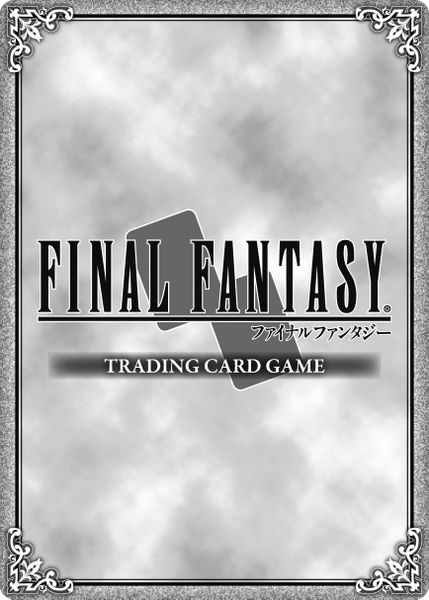
\includegraphics[width=57mm, height=79mm]{not-found.jpg}%
        \llap{%
            \raisebox{78mm}{%
                \resizebox{49mm}{\height}{%
                    \textsc{\detokenize{#1}}%
                }%
            }%
            \hspace{5mm}%
        }%
    }%
}

\begin{document}

    \noindent
    \card{15-139S_fr}%
\card{15-139S_fr}%
\card{15-139S_fr}%
\\[-0.34mm]
\card{15-131S_fr}%
\card{15-131S_fr}%
\card{15-131S_fr}%
\\[-0.34mm]
\card{15-132S_fr}%
\card{15-132S_fr}%
\card{15-132S_fr}%
\\[-0.34mm]
\card{15-133S_fr}%
\card{15-133S_fr}%
\card{15-133S_fr}%
\\[-0.34mm]
\card{15-134S_fr}%
\card{15-134S_fr}%
\card{15-134S_fr}%
\\[-0.34mm]
\card{9-062H_fr}%
\card{9-062H_fr}%
\card{9-062H_fr}%
\\[-0.34mm]
\card{1-016C_fr}%
\card{1-016C_fr}%
\card{10-007H_fr}%
\\[-0.34mm]
\card{10-007H_fr}%
\card{10-007H_fr}%
\card{10-009C_fr}%
\\[-0.34mm]
\card{10-009C_fr}%
\card{10-009C_fr}%
\card{1-105C_fr}%
\\[-0.34mm]
\card{1-105C_fr}%
\card{1-105C_fr}%
\card{5-082C_fr}%
\\[-0.34mm]
\card{5-082C_fr}%
\card{5-082C_fr}%
\card{8-085C_fr}%
\\[-0.34mm]
\card{8-085C_fr}%
\card{9-071C_fr}%
\card{9-071C_fr}%
\\[-0.34mm]
\card{9-071C_fr}%
\card{1-011C_fr}%
\card{1-011C_fr}%
\\[-0.34mm]
\card{2-005C_fr}%
\card{2-005C_fr}%
\card{5-017C_fr}%
\\[-0.34mm]
\card{5-017C_fr}%
\card{11-010C_fr}%
\card{11-010C_fr}%
\\[-0.34mm]
\card{6-075R_fr}%
\card{6-075R_fr}%
\card{6-075R_fr}%
\\[-0.34mm]
\card{6-017C_fr}%
\card{6-017C_fr}%
\card{6-017C_fr}%
\\[-0.34mm]


\end{document}


% the contents of cards.tex are generated by a script and should look something like this:

% \card{15-139S}%
% \card{15-139S}%
% \card{15-139S}%
% \\[-0.34mm]
% \card{15-138S}%
% \card{15-138S}%
% \card{15-138S}%
